% This is LLNCS.DEM the demonstration file of
% the LaTeX macro package from Springer-Verlag
% for Lecture Notes in Computer Science,
% version 2.4 for LaTeX2e as of 16. April 2010
%
\documentclass{llncs}
%
\usepackage{makeidx}  % allows for indexgeneration
\usepackage{epsfig}
\usepackage{subfigure}
\usepackage{calc}
\usepackage{amssymb}
\usepackage{amstext}
\usepackage{amsmath}
%\usepackage{amsthm}
\usepackage{multicol}
%\usepackage{pslatex}
\usepackage{apalike}
\usepackage{graphicx}
\usepackage{listings}
\usepackage{url}
\newtheorem{observation}{Observation}
\usepackage{zed}
\usepackage{algpseudocode}
%\usepackage[pdftex]{hyperref}
\DeclareGraphicsExtensions{.pdf,.png,.jpg}

\def\composition{{\mathrel{\oplus}}}
\def\optional#1{#1 [0\upto 1]}
\def\Mu{\mu}
\def\ms#1{{#1}}
\def\PA{\ms{PA}}
\def\PC{\ms{PC}}
\def\op{\underline{\smash{{op}}}}
\def\sor{\mathrel{\mathsf{or}}}
\def\orElse{\mathrel{\mathsf{or}}}
\newlength\zedminipagewidth
% we define a set of macros for constants of type 'Kind' 

\def\datamodel{\mathsf{datamodel}}
\def\dataclass{\mathsf{dataclass}}
\def\dataelement{\mathsf{dataelement}}
\def\enum{\mathsf{enum}}
\def\enumeration{\mathsf{enumeration}}
\def\primitivetype{\mathsf{primitivetype}}
\def\datatype{\mathsf{datatype}}
\def\tag{\mathsf{tag}}
\def\dataitem{\mathsf{dataitem}}
\def\abstractitem{\mathsf{abstractitem}}

% and for multiplicity 

\def\optional{0{\upto}1}
\def\mandatory{1{\upto} 1}
\def\many{0{\upto}*}

% partial ordering on constraints

\def\Cimplies{\mathrel{\implies_c}}
\def\Ciff{\mathrel{\iff_c}}

%  partial ordering on text

\def\Timplies{\mathrel{\implies_t}}
\def\Tiff{\mathrel{\iff_t}}

% and conjunction 
\def\Tand{\mathrel{\land_t}}
\def\TAnd{\mathop{\land_t}}
% our globalised version of the defining relations
\def\refines{\mathrel{refines}}
\def\newVersionOf{\mathrel{newVersionOf}}
\def\extends{\mathrel{extends}}
\def\contains{\mathrel{contains}}
% we may have \sqsubseteq and \gg when it comes to analysis 
% our two status values 
\def\draft{\mathsf{draft}}
\def\final{\mathsf{final}}
%load any additional packages

\newcommand\Algphase[1]{%
	\vspace*{-.7\baselineskip}\Statex\hspace*{\dimexpr-\algorithmicindent-2pt\relax}\rule{\textwidth}{0.4pt}%
	\Statex\hspace*{-\algorithmicindent}\textbf{#1}%
	\vspace*{-.7\baselineskip}\Statex\hspace*{\dimexpr-\algorithmicindent-2pt\relax}\rule{\textwidth}{0.4pt}%
}

%\newtheorem{definition}{Definition}
\newcommand{\Lagr}{\mathcal{L}}

%
\begin{document}
%
\frontmatter          % for the preliminaries
%
\pagestyle{headings}  % switches on printing of running heads
\title{A Data Modelling Language with Semantics and Provenance}

\author{Jim Davies \and
	David Milward}

\institute{Oxford University, Oxford, U.K.}
	

\maketitle

\begin{abstract}
An adequate account of data semantics and provenance is important in data management and analysis: to facilitate re-use and help ensure compliance.  This importance increases with the value and the complexity of the data.  This paper introduces a simple data modelling language that can be used also for the capture of semantics and provenance.  It introduces also a toolset, built around the notion of a metadata catalogue, to enable the effective deployment of the language in large organisations and major programmes.  The paper presents a language definition, using the widely-used Eclipse Modeling Framework, together with a design for the catalogue.  It reports on the experience of deploying the language and toolset in two different application domains.
\end{abstract}
%

%
\section{Introduction}

Large organizations tend to have large numbers of data flows within them, some are real-time between different applications or machine actors, which we term \emph{primary data flows} and some are reports, documents and forms which are sent between human actors, these we term \emph{secondary data flows}. Very often business process consists of data flows being transfered and stored on multiple systems and applications, with very little ability to trace or classify what data is being handled.

Abstractions are used in computer science as well as many other disciplines to reason about complex systems, and when systems are designed or reasoned about an abstraction or model will often be used.  Most object oriented software applications are designed with some regard to modelling the key aspects of the application using models and notations such as UML or Ecore.  In the same way most database oriented software applications are constructed using the entity-relationship models. Linked data systems are built using RDF models, and XML dataflows are normally designed using XML Schema. However dataflows can be in many different formats, unstructured text, comma-separated varible files, XML files, binary data standards such as ASTERIX (which is used by Eurocontrol and thus by all air traffic in Europe) and Excel spreadsheets. In both the healthcare and fintech organizations we have looked at Excel is by far the most popular application and format for sending information within the organization and for defining other data formats.

There are tools which are designed to overcome these problems, in particular Enterprise Services Buses (ESB) are used in many organizations to try and achieve interoperability between different services. Such toolkits rely on all participants using a common \emph{service oriented architecture}, and to a point these systems work very well assuming all the software components using the system are configured as services, and use one of the protocols mandated by the toolkit in question.  Our experience in both Healthcare and FinTech indicates that most operational environments ESB technology cover only a relatively small percentage of the dataflows, and that many issues of data provenance and semantics are still present

A Metadata Registry is a toolkit which allows definitions of datasets to be stored, curated and managed. The definitions are metadata, and could be the decription of a field in a relational database, or an element in an XML file. By storing the definitions of every data element and all its relations in a metadata registry the map of all the dataflows in an organization can be created and managed. It is similar to an ESB. an in fact most ESB's have some kind of registy internally to hold metadata. Metadata Registries, such as those conforming to the ISO11179 standard, can help to solve the problem of data incompatibility, provenance and compliance, as is indicated in studies such as those conducted by Ulrich et al. \cite{MDRHL7} . In this study a hybrid architecture consisting of an ISO 11179-3 conformant MDR server application for interactively annotating and mediating data elements and the translation of these data elements into FHIR resources was used to manage data for the North German Tumour Bank of Colorectal Cancer. 

The ISO11179 standard allows complex mapping between data elements, conceptual domains and value domains; however it does not have a mechanism which allows data elements to be easily grouped into hierarchical components, such as are found in most datasets and dataflows. There are two mechanisms defined in ISO11179 for grouping data elements, one is \emph{classifications} and the other is \emph{object properties}, however neither allows for any kind of grouping or componentization of the kind which is found in UML, ERM or XSD. As a result integrating ISO11179 in legacy software systems requires extra work and mapping and therefore many of the issues addressed by the standard are complicated rather than simplified when applying the standard to the design of a metadata registry. 

In this work we have taken the core elements in ISO11179, and built an Ecore model which attempts to overcome these problems, and in doing so we have defined a simple language for metadata management.


\section{Background}

Much of the patient data collected in the U.K.'s National Health Service (NHS) remains unaccessible for medical research. This is because it is held in a variety of commercial software systems which have been built at different times, and have been based on different standards. Reporting consists largely of data being sent in excel spreadsheets, csv files or xml files.  There are over 130 different data models and standards (see TRUD \cite{TRUD}) currently being used in the NHS at present, and new ones are being introduced and implemented each year. At present the UK NHS is preparing to implement SNOMED across all systems by 2020, this has largely been achieved in primary care, but has hardly been started in secondary care systems. The main reason for the success in primary care is down to the fact that there are 5 main vendors of primary care systems, all of whom regard the UK primary care market as a major part of their business, and hence all of them have agreed to implement the standard.  

However in secondary care the larger hospital trusts will be running 2-300 different systems, many of these from vendors with bases outside the UK, who have little incentive to make major changes to systems which they are selling in a minority marketplace. Efforts by the core standards bodies within the NHS to impose standards on hospital truests have met with partial success. As well as the technical challenges, there are also legal issues imposed by the Health and Social Care Act 2012, NHS Act 2006, the Health and Social Care Act 2012, the Data Protection Act 1998, the Human Rights Act, and the shortly to be introduced General Data Protection Regulations.  The complexity of these different acts results can result in data on a patients other conditions (say liver disease) being withheld from Emergency Care Clinicians when they are performing for instance emergency heart surgery. Whilst such legislation clearly is intended to protect the patient's privacy, it can have unforseen side effects not only on emergency medical care, but also on the ability and ease in which medical data can be aggregated for further research purposes.

Medical data when aggregated is generally stored in relational databases, excel spreadsheets or unstructured pdf and word documents, and querying this data can be very difficult in all these cases. Reports are sent through to the NHS from local hospital trusts to satisfy reporting requirements in hundreds of different spread-sheet formats, with no real verification on the datasets contained. There is no question that the information \emph{could} be valuable for research, however extracting data for analysis is very often too costly to perform.  When datasets are prepared for analysis it is often discovered that the structure of the data when stored may not be the same as the structure it is required in now, and there maybe no exact record of how the data was originally recorded. For instance gender may be stored in one system as an enumeration of \emph{yes or no} and in another system as \emph{yes, no, unknown}, if we write a query assuming the former then we may arrive at incorrect conclusions if the data is actually collect in the format of the latter, but assumed to be conforming to the former. 

The work described here started with the development of an ISO11179 for the CancerGrid project~\cite{davi14}, in this work an ISO11179 metadata registry was built to curate datasets for clinical trials data, and to develop clinical trials software~\cite{davi12, Abler2011}. This work was informed by previous initiatives to implement an ISO11179-compliant registry in the CaBIG initiative, which was used to generate code for web service stubs.

\section{Language}

This metamodelling langauge (MML) is constructed for data interoperability and it has a metamodel \textbf{$M_2$} defined at level M2 of MOF. The language can be designated by $\Lagr_{m2}$ and a meta-model ML is formally defined by this language $\Lagr_{m2}$.

It is aimed at Information Systems, which are simply storing and handling data, so at present we are not looking at having the language capture \emph{behaviour}, it is simply a \emph{structural meta-language} for describing data items. 

Most information systems use a variety of mechanisms to store data, from text files to relational databases, all of which can be modelled at the M1 level.  In fact we can say that the M1 languages which model the data can be designated by $\Lagr_{m1}$, each one defining a Model which we can designate by MI = (mi\_1, mi\_2, ...., mi\_n).  MI being the collection of Models that \emph{conform to} or \emph{implement} MML.  

An example of a \emph{Data Language (say mi\_1)} at this M1 level of abstraction would be the UK NHS's Cancer Outcomes and Services Dataset (COSD) which is a dataset specifying the terminology to use when writing reports on cancer. At present the dataset is defined by both an excel file and an XSD.  Within the NHS there are plenty of other similar datasets, which are used in reports, in databases or by applications.  Whilst MML will not be a fit for every dataset, it is aimed at covering most structural features that occur in datasets, it can be viewed as a subset of Ecore tailored to the domain of data management.

In defining MML we take the notion of a \emph{dataElement} as the core entity in the language, historically it was intended to correspond to a \emph{data element} in ISO11179 and with an \emph{element} in the UML meta-model. It is an atomic data item, capturing one single element that cannot be sub-divided.

The word or stem \emph{abstract} is used in several different ways in this discussion, and the following brief discussion highlights the different usages.  

Firstly we can have an abstract entity which is the implementation of an EClass at the M3 level, that is to say a representation of in our language of an EClass which cannot be implemented at the M2 level. It can be \emph{sub-typed} by another EClass at the M2 level and this \emph{sub-class} can be implemented. We use this mechanism to specify both AbstractItem and DataItem as \emph{abstract} entities in our language, however we are not defining an \emph{abstraction} mechanism for MML per se. Later on we will define an inheritance or rather a simple sub-typeing mechanism which can be used for \emph{templating} at the M1 model level. 

Secondly we are referring to each layer as being an \emph{abstraction} of the previous layer, and therefore having less concrete description, this is the notion built into the idea of MOF layers. 

\begin{figure}
	\centering
	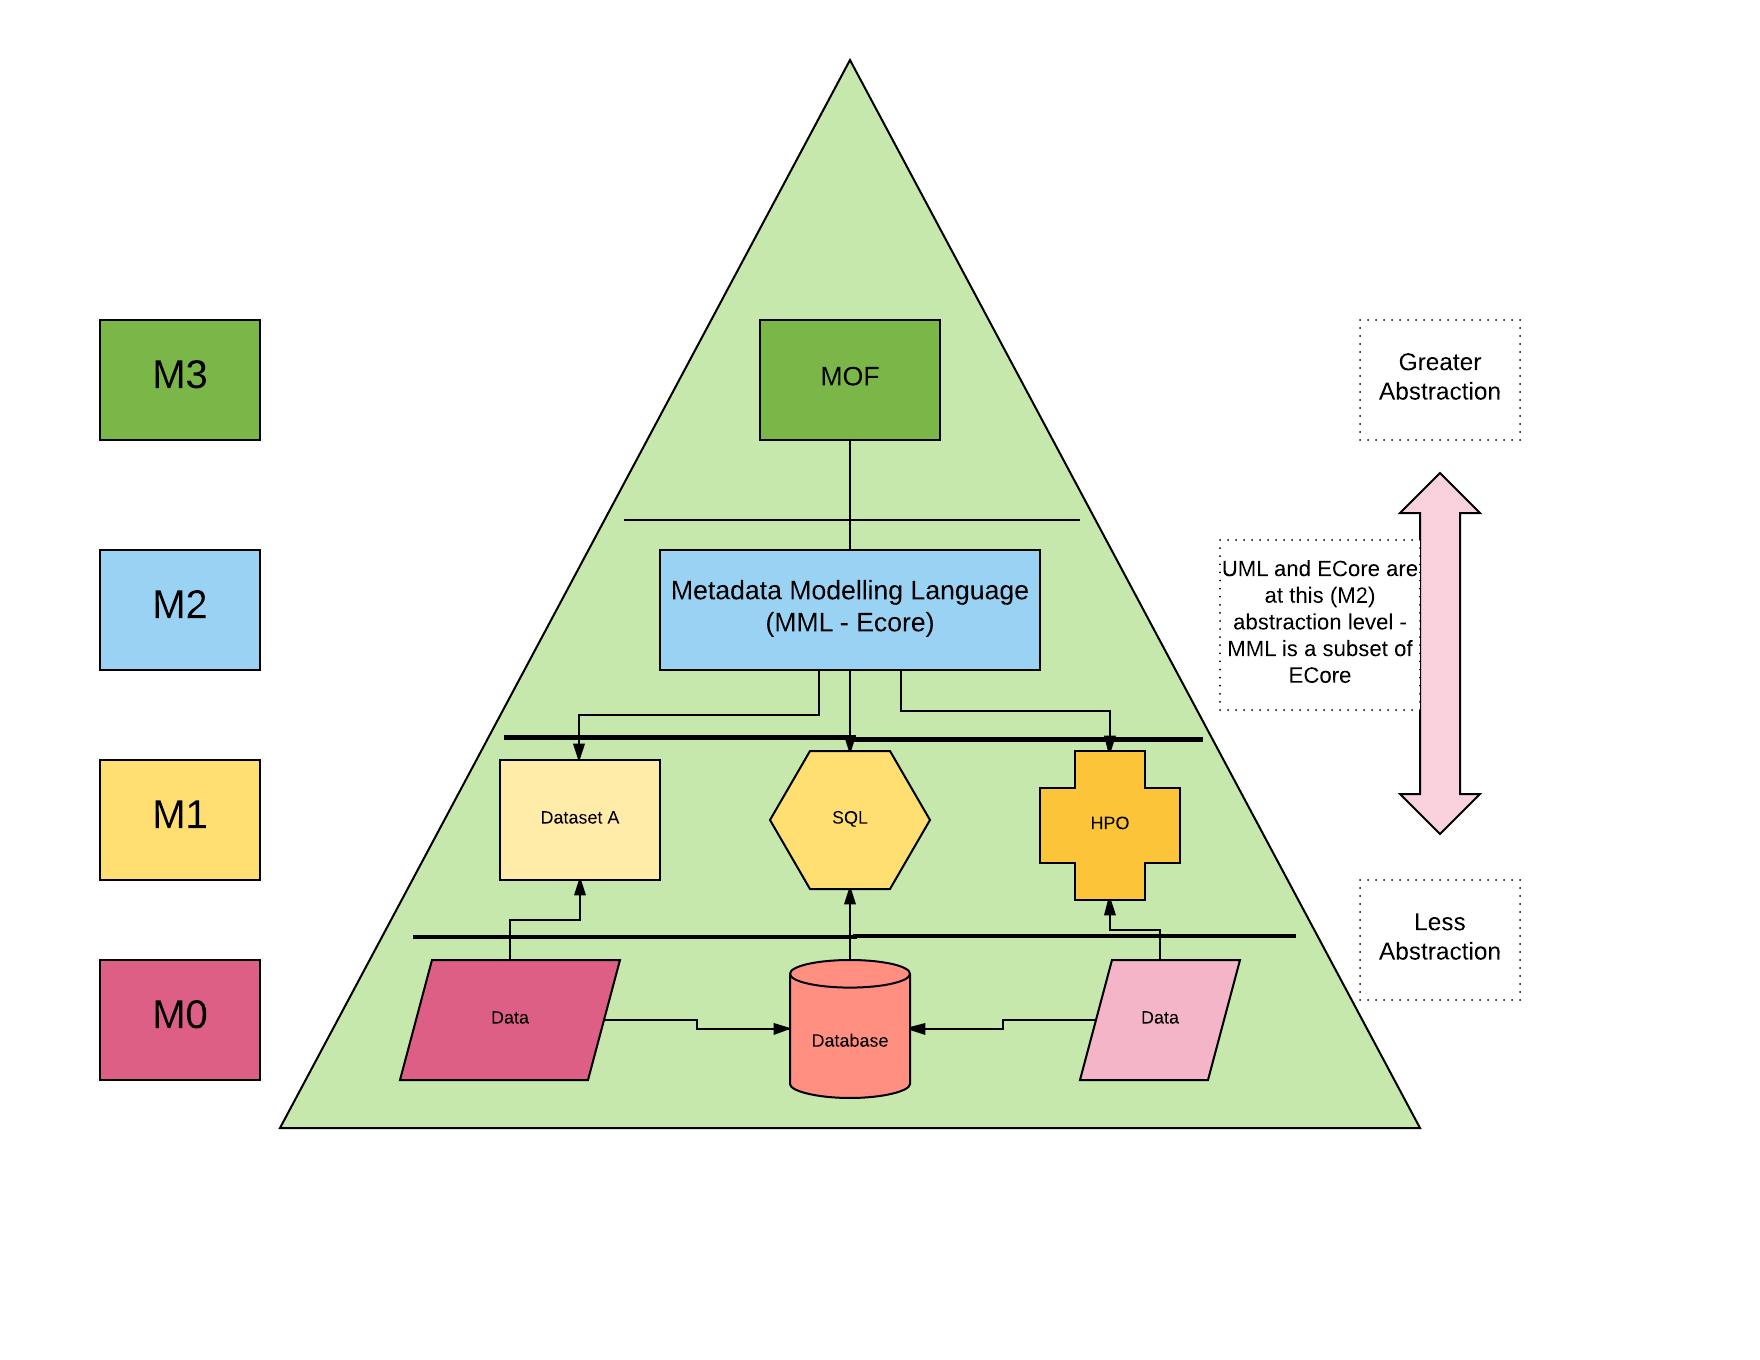
\includegraphics[scale=0.45]{figures/MMLMOFModel}
	\caption{MOF and MML}
	\label{fig:mofmml}
\end{figure}



\subsection{Language Definition}

\subsubsection{Core Elements of MML}

\subsubsection{Core Elements of MML}

\subsubsection{MML Grammar}

The following section shows the code used to define the XText grammar, which is used to generate an Ecore meta-model, which in turn is used to define the different datasets used in this project.
\begin{small}
	\begin{verbatim}
	grammar uk.ac.ox.cs.MML with 
	org.eclipse.xtext.common.Terminals
	
	generate mML "http://www.ac.uk/ox/cs/MML"
	
	MML :
	(elements += AbstractItem)*
	;
	
	
	DataModel:
	'DataModel' name = QualifiedName '{'
	(elements += AbstractItem)*
	'}'
	;
	
	AbstractItem:
	DataModel | DataClass | DataType | Import
	;
	
	QualifiedName:
	ID('.' ID)*
	;
	
	Import:
	'import' importedNamespace = 
	QualifiedNameWithWildcard
	;
	
	QualifiedNameWithWildcard:
	QualifiedName '.*'?
	;
	
	
	DataType:
	'DataType' name = ID
	;
	
	ContainerElement:
	DataClass| DataElement
	;
	
	DataClass:
	'DataClass' name = ID ('extends' superType =
	[DataClass])? '{'
	(dataelements += ContainerElement)*
	'}'
	;
	
	DataElement:
	'DataElement' name = ID ':' type =  
	[DataType|QualifiedName]
	;
	\end{verbatim}
\end{small}



\subsection{Language Properties}


\section{Application}


\subsection{Health Service Example}
\subsection{FinTech Example}


\section{Conclusion}





%\bibliographystyle{IEEEtran}
\bibliography{CAISE2018}


\end{document}
